\subsubsection{Comparisson to the analytical solution}
\begin{figure}[h!]
    \centering
    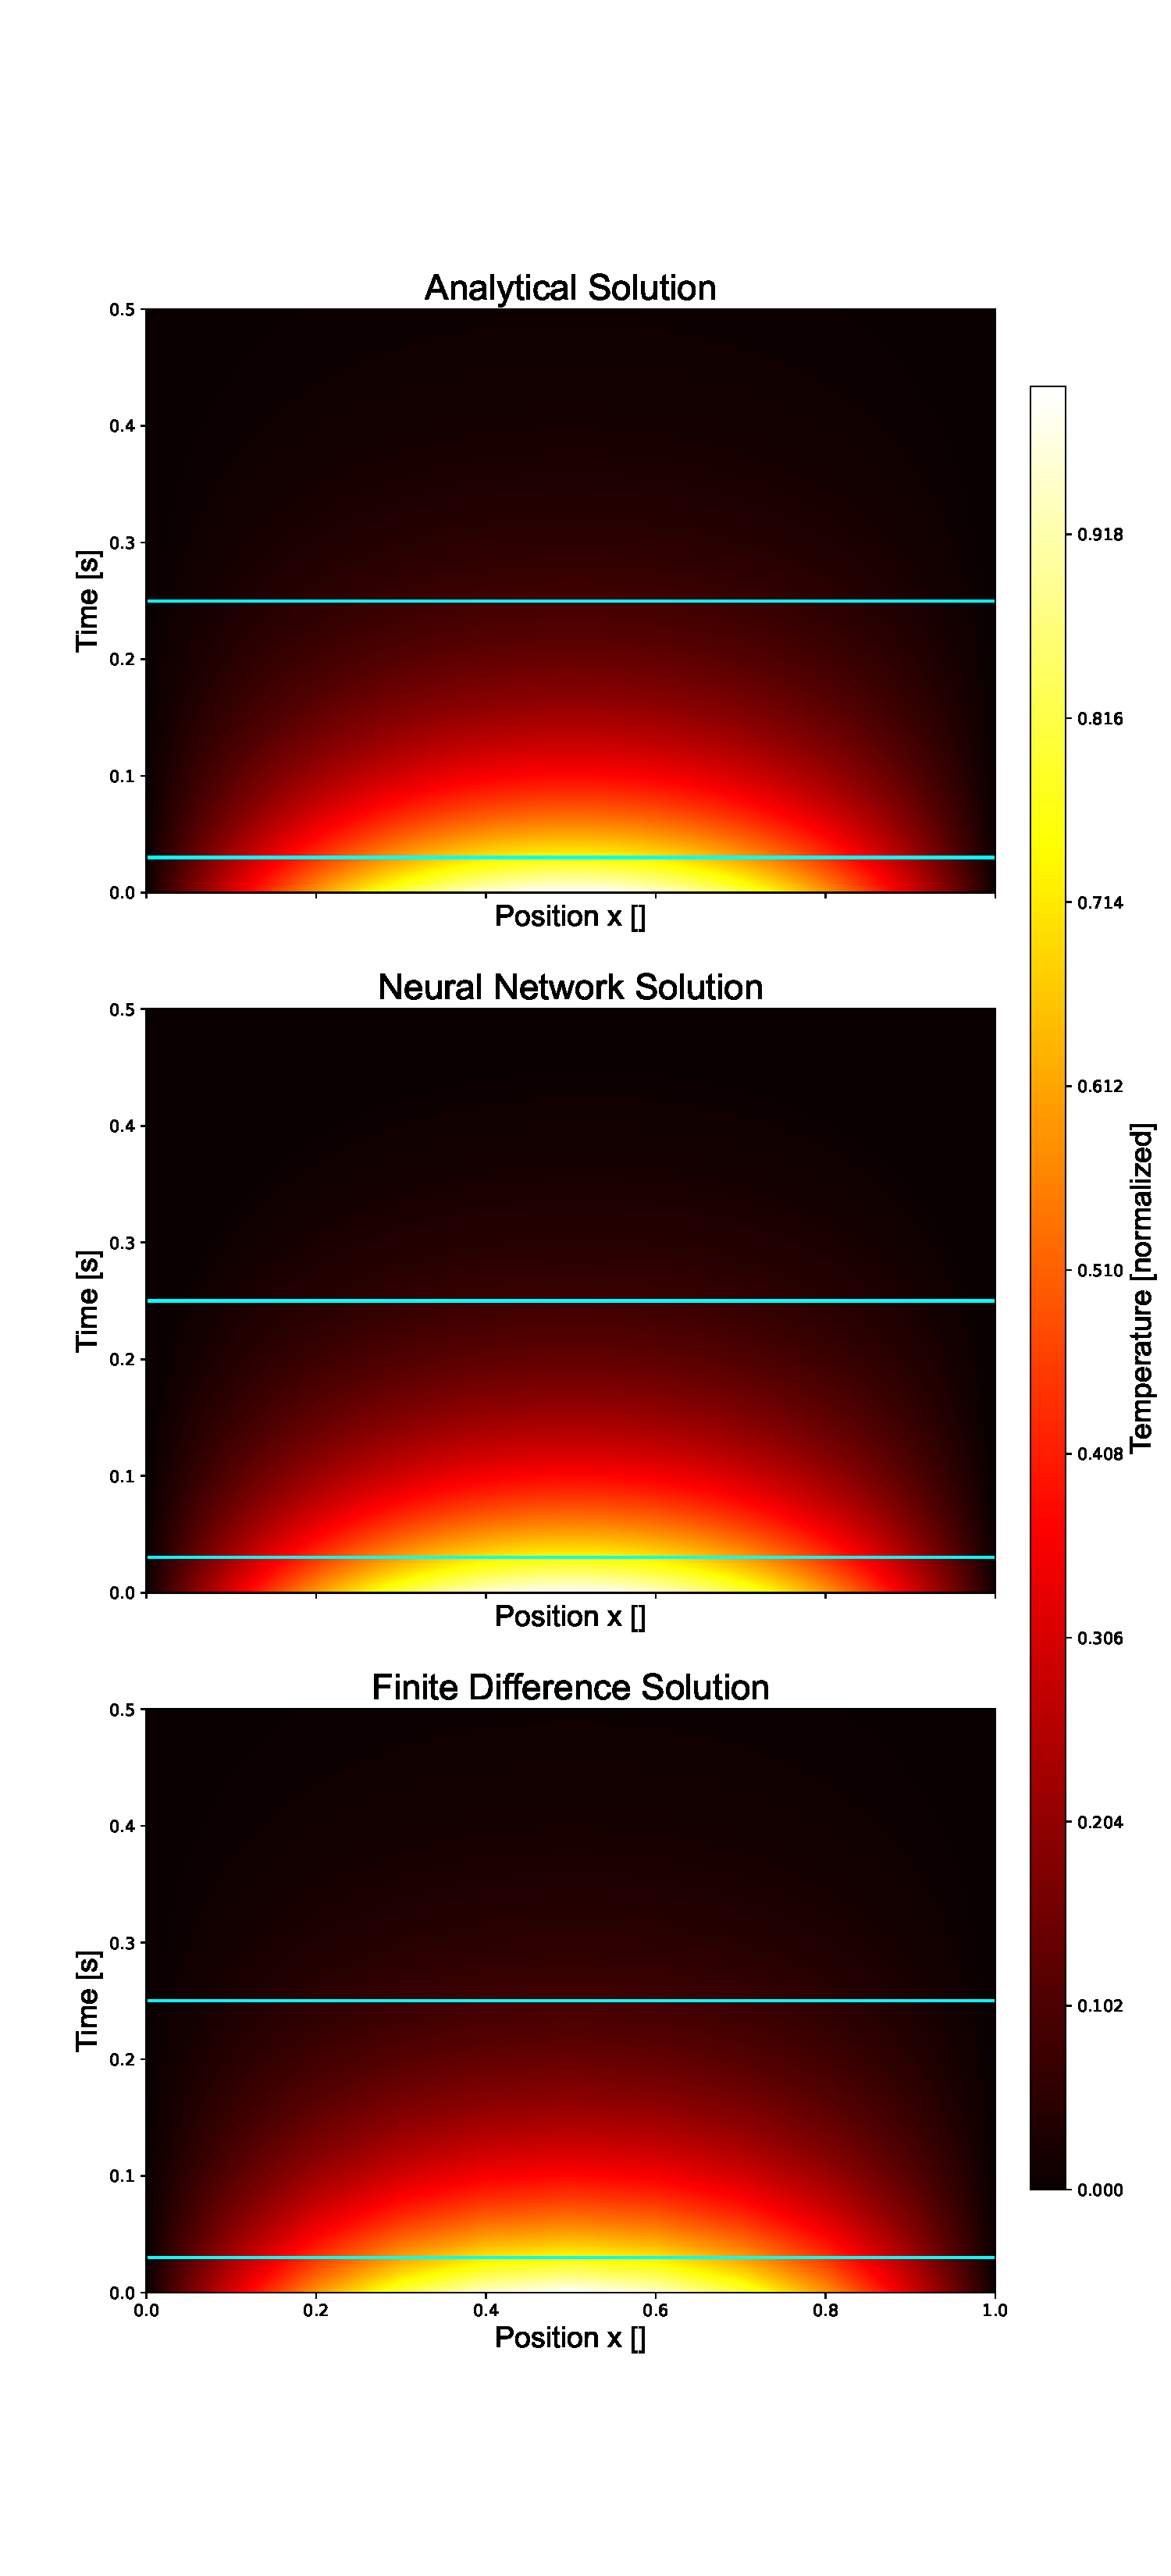
\includegraphics[width=1.0\linewidth]{project_3/plots/heat_map_comparison.png}
    \caption{The analytical solution to the heat equation, and the results from the finite difference method and the neural network model. A common color bar is displayed as all three plots have the same range of values [0,1]. The blue lines indicate the times $t_1 = 0.03 s$ and $t_2 = 0.25 s$.}
    \label{fig:heatmaps}
\end{figure}

The results from the finite difference method and the NN are presented in Fig. \ref{fig:heatmaps}.
In this plot, the outputs from the finite difference models have been interpolated making them appear smooth even though the model only outputs a discrete set of values. 
There is no noticeable difference by eye between the three plots, which is well reflected in the very low MSE-value observed in both numerical methods. 
Compared to the analytical solution, the output of the neural network model has an MSE of $ 6.71 \times 10^{-6}$ while the finite difference method yields an MSE of $2.52 \times 10^{-7}$. 
Since the two methods utilize different discretizations of the $(x,t)$ grid, the analytical solution is evaluated only at the respective grid points of each method. 
Consequently, the MSE calculation for the neural network involves a greater number of points than that of the finite difference method.
As the finite difference model only provides predictions for a predefined set of discrete points, it does not make sense to calculate its MSE on a set of points with finer granularity.
However, the resolution of points used to calculate the MSE will not have a substantial impact on its value, hence the MSE values are still comparable.
\begin{figure}[h!]
    \centering
    \includegraphics[width=1.0\linewidth]{project_3/plots/time_slices_comparison.pdf}
    \caption{The temperature for specific times for the analytical solution, as well as the output from the finite difference method and the neural network predictions. The discretization along the x-axis is different for each method. The analytical one is plotted with 1000 points, the finite difference method with 11 points, and the neural network predictions with 100. }
    \label{fig:timeslices}
\end{figure}


We ``\textit{slice}" the heatmaps in Fig. \ref{fig:heatmaps} at two specific times, $t_1 = 0.03 s$ and $t_2 = 0.25 s$. 
This is illustrated as blue lines in Fig. \ref{fig:heatmaps}.
The temperature values across the x-range are plotted for all three cases in Fig. \ref{fig:timeslices}.
At $t_1$, the function is still significantly curved, while at $t_2$ it has almost reached the stationary state.
This serves as an additional verification of the previously presented results. 
The finite difference method seems to match the analytical solution to a high accuracy in its discrete points, while the neural network is slightly undershooting.
The effect of this is more prominent for the later time stamp $t = 0.25 s$. 
These results reflect well the lower MSE for the finite difference method compared to the NN. 
\mia{The reason for this might be: }

\subsubsection{Finite difference method}

\mia{Additionally, the finite difference method with 100 points along the x-axis is plotted to illustrate what???}

\mia{why is N = 10 and N = 100 equally good for fd?}

\gaute{numberos}


\subsubsection{Exploration of the hyperparameters of the neural network}

The results from the in-depth investigation of the impact of the hyperparameters \textit{number of hidden layers}, the \textit{size of the hidden layers}, and the \textit{activation functions} are presented in Figs. \ref{fig:boxplots_activations}, \ref{fig:boxplots_size_of_layers} and \ref{fig:boxplots_number_of_hidden_layers} respectively. 
From the three-dimensional grid search, the best values were found to be three hidden layers with size 50 and tanh as the activation function.


\begin{figure}[h!]
    \centering
    \includegraphics[width=1.0\linewidth]{project_3/plots/activation_search.pdf}
    \caption{Boxplots showcasing the final MSE value compared to the analytical solution for different activation functions. Each model is run 10 times.}
    \label{fig:boxplots_activations}
\end{figure}

%Mean MSE for activation = leakyReLU: 0.34531696140766144
% Mean MSE for activation = ReLU: 0.3466638922691345
% Mean MSE for activation = tanh: 1.579682736974064e-05
% Mean MSE for activation = sigmoid: 0.010715706355404109

As activation functions, sigmoid and tanh outperform ReLU and leakyReLU. 
The two former force the raw output from a node to a set range of values, $(0,1)$ and $(-1,1)$ respectively. 
The variants of ReLU, however, do not truncate the high positive values of the outputs from the nodes. 
Given the nature of the problem, it is highly intuitive that the ReLU-variants perform poorly. 
The output is known to be in the range [0,1]. 
Therefore, it is interesting to discuss why tanh does better than sigmoid, given that the ladder yields output in the same range. 
\mia{that is only for the hidden layer nodes, the output layer activation function is identity}
\mia{The sigmoid never gives zero exactly and a lot of our canvas is close to zero in value}
\mia{why}

\begin{figure}[h!]
    \centering
    \includegraphics[width=1.0\linewidth]{project_3/plots/value_layers_search.pdf}
    \caption{Boxplots showcasing the final MSE value compared to the analytical solution for different sizes for the hidden layers. Each model is run 10 times. }
    \label{fig:boxplots_size_of_layers}
\end{figure}

% Mean MSE for value_layers = 10: 0.0012251243981154403
% Mean MSE for value_layers = 25: 2.3295253322430652e-05
% Mean MSE for value_layers = 50: 1.579682736974064e-05
% Mean MSE for value_layers = 100: 3.0093467512415372e-05

The size of the hidden layers dictates the width of the NN. 
In Fig. \ref{fig:boxplots_size_of_layers} one can see that a size of 10 is producing the poorest result, suggesting the NN does not capture the complexity of the problem with this. 
The other are harder to distinguish by eye and we therefore present the mean MSE for each of them. 
For hidden layers of size $25$ the MSE is $2.32 \times 10^{-5}$, for $50$ the MSE is $1.57 \times 10^{-5}$ and lastly, for 100 it is $3.00 \times 10^{-5}$.
There is an increase in performance as the width of the NN increases up to $50$. 
After this, however, the network seems to be overfitting \mia{to what???}. 

\begin{figure}[h!]
    \centering
    \includegraphics[width=1.0\linewidth]{project_3/plots/n_layers_search.pdf}
    \caption{Boxplots showcasing the final MSE value compared to the analytical solution for different numbers of hidden layers. Each model is run 10 times.}
    \label{fig:boxplots_number_of_hidden_layers}
\end{figure}

% Mean MSE for n_layers = 1: 0.012613625824451446
% Mean MSE for n_layers = 2: 0.0004955611351761035
% Mean MSE for n_layers = 3: 1.579682736974064e-05

The number of hidden layers dictates the depth of the NN. 
As seen in Fig. \ref{fig:boxplots_number_of_hidden_layers} one hidden layer yields the highest mean MSE among the tested numbers. 
Both two and three hidden layers (with a size of 50 for each) perform way better, suggesting more layers are necessary to properly capture the complexity of the task. 
While two hidden layers yield an MSE of $4.96 \time 10^{-4}$, three gives $1.58 \times 10^{-5}$, a factor 19 lower. 


We could have tested for four hidden layers in our grid search. 
However, this would have required way more computational time, and seeing as the NN model matches the analytical solution well, this was found not to be necessary and remains a topic for future investigations. 
Similarly, zero hidden layers (corresponding to a linear regression model) was not tested \mia{because ...}